%%%%%%%%%%%%%%%%%%%%%%%%%%%%%%%%%%%%%%%%%%%%%%%%%%%%%%%%%%%%%%%%%%%%%%%%%%
%                                                                         %
%      This file is part of the 'openLilyLib' library.                    %
%                                ===========                              %
%                                                                         %
%              https://github.com/lilyglyphs/openLilyLib                  %
%                                                                         %
%  Copyright 2012-13 by Urs Liska, lilyglyphs@ursliska.de                 %
%                                                                         %
%  'openLilyLib' is free software: you can redistribute it and/or modify  %
%  it under the terms of the GNU General Public License as published by   %
%  the Free Software Foundation, either version 3 of the License, or      %
%  (at your option) any later version.                                    %
%                                                                         %
%  This program is distributed in the hope that it will be useful,        %
%  but WITHOUT ANY WARRANTY; without even the implied warranty of         %
%  MERCHANTABILITY or FITNESS FOR A PARTICULAR PURPOSE. See the           %
%  GNU General Public License for more details.                           %
%                                                                         %
%  You should have received a copy of the GNU General Public License      %
%  along with this program.  If not, see <http://www.gnu.org/licenses/>.  %
%                                                                         %
%%%%%%%%%%%%%%%%%%%%%%%%%%%%%%%%%%%%%%%%%%%%%%%%%%%%%%%%%%%%%%%%%%%%%%%%%%%

\documentclass[../../LilyPond-Tutorials]{subfiles}

\begin{document}
\parttitle[Urs Liska]{Plain Text Files in Music}
\begin{authorAbstract}{Urs Liska}
The idea of editing plain text files when creating musical scores and text documents may seem strange to people used to working with graphical tools.
But there are serious advantages going the route of plain text driven workflows---starting from superior result quality, extending through robust and reliable storage forms, up to workflow options unimaginable otherwise.

This paper introduces musicians and musicologists to key concepts of working with plain text documents and collaborative workflows.
In particular it deals with the LilyPond notation software, the \LaTeX{} typesetting system, and version control.

\end{authorAbstract}

\chapter*{Introduction}
\label{chap:pt_introduction}
This paper discusses an approach to authoring musical documents%
\footnote{i.\,e.\ scores and texts about music}
that is based on editing \emph{plain text files} instead of using graphical \textsc{wysiwyg} software%
\footnote{What You See Is What You Get---such programs provide an editing environment where the document is displayed identically to the way it will be printed.}.
The described concepts, tools, and workflows have significantly changed my life as a document author, and I  wholeheartedly endorse them because I strongly believe in their unique and substantial advantages.

The plain text approach is practically non-existent in the humanist disciplines or in the music business, while being de facto standard in many natural and computer sciences.
Working with plain text based tools indeed requires a certain shift in mind-set for people who aren't already familiar with the corresponding working paradigms.
And it can't be denied that the learning curve is considerable.
But this investment is absolutely justified because on the long run it greatly benefits productivity and offers potentials unimaginable otherwise.
Reading and writing music, playing an instrument, investigating a manuscript source---all this involves a very long and intense learning curve, and we mastered them as a matter of course in order to become the professionals we are.
Don't be afraid to learning something new!

% i think the introduction was getting too long.

This document aims to give you an overview of the
power that text based approaches can give you.
It is not meant as a detailed description or a guide
to using the software mentioned --- for that, please refer
to the suggested reading at the end.

The software packages I will introduce you to on the following pages are:
\begin{itemize*}
\item \emph{LilyPond} -- the program that lets you engrave beautiful scores
\item \emph{Git} -- the versioning system that keeps your work under control
\item \emph{\LaTeX} -- the professional typesetting engine for text documents
\end{itemize*}

\chapter{Plain Text Format}
\label{chap:pt_plain-text-format}
Who on earth would voluntarily enter music as a text file?
Aren't these people just nerds who think that only what hurts can be good?
Isn't it \emph{natural} to edit musical scores within a graphical user interface?

Well, a graphical user interfaces which allow users to edit
a document with a mouse or other pointing device is obviously
quick, effective and easy.
However, there are lots of reasons why it \emph{is} a good idea to edit and store documents in text files.
Text based work avoids several fundamental problems that other approaches share, and it opens up a whole range of advanced options not imaginable otherwise.
And it is good to know that by now there are editors available that significantly assist you in dealing with text files.

Firstly, let us consider a number of features of working with plain text files.

\section{Transparency and Control}
\label{sec:pt_transparency-and-control}
Have you ever wondered how your notation program internally manages the contents you entered, especially when you had the impression it maliciously made fun of you?
One of the reasons I turned my back on graphical notation programs was my frustration with being completely at the mercy of the software with regard to my personal layout decisions.
I can't recall (and actually don't want to) how often I ran through the loop of
\begin{inparaenum}[1.)]
\item entering music,
\item moving items around ,
\item applying some manual tweaks like flipping stems, breaking beams, suppressing or parenthesizing cautionary accidentals,
\item hitting “Update Layout” and finally
\item tearing my hair out because at least one third of my manual settings mysteriously vanished.
\end{inparaenum}

It's been a long while since I had used graphical software, so maybe things have improved a lot, but the fundamental fault is still valid: 
I am at the mercy of the software and can't see or control how it represents the content internally.

A friend finally stopped using (a later version of) the same graphical program when he fixed one missing accidental in a score he had earlier tweaked to perfection---and this accidental caused the whole layout to break irreversibly.

Besides this risk of losing work I also can't usually tell how the program
interprets changes I've made.  For example, if I add a description text
somewhere near the violin staff, will it follow the music when the page layout
changes or will it stay in the same position relative to the corner of the page?

\medskip
\todo{Example how this applies to text documents}

\medskip
If I edit a plain text file instead I'm completely in control over all these issues.
If I tell the program to break a beam or to draw a slur above the note it is explicitely and reproducibly defined and readable by anybody.
There is nothing hidden in “settings” dialogs or even unreadably buried somewhere in the file as the result of dragging something with the mouse.
If I manage to break something (which of course happens) I can review what I did, compare to the last working version%
\footnote{See the “version control” \fref{chap:pt_version-control}}
and understand and fix the issue.
With a graphical program my only resort is to “undo” and hope this will fix it \dots

There is a price for this, namely having to enter code by hand and learning how to do that, but it is very rewarding on the long run.
And being in control just \emph{feels} better \dots

\section{Content, Meaning and Appearance}
\label{sec:pt_separation-content-meaning-appearance}
Through the overwhelming presence of \textsc{wysiwyg} applications we have got used to the impression that the \emph{visual appearance} of a document is identical to its \emph{content}.
But this is actually a quite shortsighted assumption.

If you look at that text document:

\begin{center}
\noindent\shadowbox{\parbox{.8\textwidth}{%
\Large \textbf{\textsf{My new chapter}}

\medskip
\normalsize \textbf{\textsf{With a section}}

\medskip
\small This is the \textbf{\textsf{continuous}} text with some \textbf{\textsf{emphasized}} words.}
}\end{center}

\noindent you will notice that there are several parts formatted in sans-serif bold face of different sizes.
You may guess that the author has applied several style sheets to get this appearance, but to verify it you'd actually have to select the texts and look into the corresponding dialogs or toolbox elements.
Only then you can see whether the author manually formatted the text, applied paragraph styles or character styles.
He may even have applied character instead of paragraph styles to format the headings.

The corresponding \LaTeX{} source file would look like:

\begin{lstlisting}[language={[LaTeX]TeX}]
\documentclass{article}
\newcommand{\terminus}{\textbf{\textsf{#1}}}
\begin{document}
    \chapter{My new chapter}
    \section{with a section}
    This is the \terminus{continuous} text with
    some \textbf{\textsf{emphasized}} words.
\end{document}
\end{lstlisting}

While this may look complicated on first sight it actually is much clearer because it distinctly shows you the content \emph{and} the author's intentions.
The \cmd{documentclass} is something like a document template, but much more powerful%
\footnote{See the \LaTeX{} chapter \fref{chap:pt_latex}}.
\cmd{terminus} is defined as a character style applying bold (“\dots bf” for BoldFace) and sans-serif (“\dots sf” for Sans-Serif) to its content (“\#1”).
Inside the document body (enclosed by the \cmd{begin} and \cmd{end} statements) you can see the \emph{content} along with \emph{semantic markup}.
The two headings use explicit sectioning commands which are (for now) equivalent to paragraph styles.
The two bold words in the text line are formatted differently: 
the first one  is enclosed by our \cmd{terminus\{\}} character style while the second one is manually formatted as bold and sans-serif.
This mixture of formatting techniques is highly disadvised and only used for the sake of the example.
But you may notice that in the plain text file this “problem” is immediately obvious while the graphical program actually hides away such inconsistencies.

\medskip
If we think about musical scores we have to come to a very similar conclusion.
I began this chapter with the rhethorical pretention that it is “natural” to edit a score in a graphical way.
But in fact that's not entirely true because a score isn't a graphical object like a painting
but rather a graphical \emph{representation} of the musical \emph{content}.

If you consider the following minimal score and its (complete) LilyPond input file:
\begin{multicols}{2}
\vfill
\begin{musicExampleNonFloat}
\begin{quote}
\lilypondSFE{examples/minimal-score}
\end{quote}
\end{musicExampleNonFloat}
\vfill
\columnbreak

\begin{centering}
\begin{lstlisting}
{
  \time 3/4
  \key es \major
  \clef bass
  es8 f8 g8 as8 f8 es8
}
\end{lstlisting}
\end{centering}
\end{multicols}

\noindent you can see that the source on the right side completely defines the \emph{musical content} of the score:
a time signature, a key definition, a clef, and a few notes with durations.
Of course the page layout is also an inseparable part of the score document, but on a conceptual level it is completely separate from the musical content.
Without going into more detail here you should note that in LilyPond's plain text file you have complete control over the separation of content, meaning and appearance.
While this at first may seem somewhat abstract it is actually a very important point when it comes to preparing different output from one source%
\footnote{See “single-source publishing” section \fref{sec:pt_single-source-publishing}}.

\section{Readability and Stability of Text and Binary Files}
\label{sec:pt_readability-stability}
In the previous section you have seen examples of plain text files for a text and a score document.
OK, I admit that it takes some time getting used to filtering out the markup commands in a text file mentally.
But I can't emphasize enough that you actually \emph{can read} that file \emph{at all}.

Does this bold statement surprise you?
Don't you think that you can immediately conceive the content of the graphical score, much faster and easier than the source file that you first have to read and interpret?
Well, then you are again exchanging the real document file and the graphical representation the graphical programs expose to you.

Please take the time and have a look at \todo{prepare “listings”, put them in appendix and add link to them}.
That's what the file contents from the previous examples actually look like.
After skimming through the Word\texttrademark, OpenOffice\texttrademark, Finale\texttrademark{} and Sibelius\texttrademark{} files you should reconsider the “overly complex” \emph{source code listings} of the previous section.
Now you'll probably see why I emphasize that you can \emph{read} \LaTeX{} and LilyPond files, isn't it?
You may have noticed that both Word\texttrademark{} and OpenOffice\texttrademark{} also have an alternative file format that is stored in “plain \textsc{xml}”.
While a human actually \emph{can} read these files the actual content is very deeply buried inside them and practically inaccessible to the human eye.
	
The fact that plain text files are human readable has two major implications:

\paragraph{Recovery after file corruption}
There are several ways that can make a file unusable, the most common being accidental deletion, a general disk failure or the crash of a program leading to an inconsistent state of the file (the latter fortunately becoming increasingly rare nowadays).
Usually such files can be partially retrieved with special tools, but the picky thing is the “partially”.
If you have a binary file that can only be read by its original program the whole file is now unusable, even if the corrupted portion is very small.
From a corrupted plain text file on the other hand you will be able to retrieve everything \emph{as content} that is still there at all.
And with some luck you may even guess the missing pieces.
Sometimes it will still be more efficient to start again from scratch, but depending on the nature of your project this characteristic of plain text files may actually be a life-saver.

\paragraph{Restoring “ancient” files}
As programs mature they modify their file formats.
Usually programs can still open the files from older program versions, but that isn't an endless option.
With the majority of programs you would need to have some older version around to be able to open “ancient” files.
And with new operating systems chances become increasingly worse to find one.
Generally speaking, when software becomes unsupported its documents tend to become unusable.

This may also happen with programs that store their data in plain text files.
But as the file format is usually much better documented it is more likely that you will find a conversion option still available.
And if everything fails and you have a file but no dedicated editor you still have the plain text and free access to it.

\section{Editor Independence}
\label{sec:pt_editor-independence}
Plain text workflows separate the tasks of editing, processing and displaying documents.
This way you are not restricted to \emph{the one} application the (commercial) vendor imposes on you, but you are free to chose any editing environment you like, consider appropriate or just feel comfortable with.
There are programs that try to integrate all parts of a workflow, just like the \textsc{wysiwyg} tools do---but it is your free choice to use them or not.

You can even edit a project with different tools at a time.
For example it might be handy to be able to edit a document with any text editor on your smartphone, or just going to a public internet access point and send yourself an email with a sketch---both of which you would then process to a pdf document when you are home again.

Another interesting application is the use of plain text as input to web forms.
Many web forms, e.\,g.\ in forums, allow you to enter your posts in \emph{Markdown}%
\footnote{\url{http://daringfireball.net/projects/markdown/}},
a minimalist plain text language, and convert them to formatted \textsc{html}.
And recently \emph{Wikipedia} added support for LilyPond code that will be rendered as music examples.

\section{Programmability}
\label{sec:pt_programmability}
Plain text files can be edited not only by any text editor but by \emph{anything} that can edit text files---which makes it accessible to about any programming language you may think of.
You are not restricted to any scripting interface the vendor graciously provides you, but you can apply any imaginable operations with your source files: 
analyze them,
process them,
or even computationally generate them from scratch.
There are many possible applications, from applying contrapuntal operations or algorithmic composition up to managing music examples in a database.

If you have never programmed and don't intend to learn it you may think that's a rather unimportant feature.
But this isn't true at all.
For example I'm currently working on the infrastructure for a large orchestral score where those who enter the music only work on small segments of the instrumental parts.
The full score (which is initially filled with rests) will automagically build itself and use whatever segments have already been entered.
This is an example of an approach where the administrators of a project \emph{explicitely} use programming to allow sophisticated logic in the project while at the same time hiding the complexity from the regular contributors.


\section{Compiling Files vs.\ Instant Feedback}
\label{sec:pt_compiling-instant}
One thing the average \textsc{wysiwyg} user needs to get used to is \emph{not} to get instant feedback.
Graphical programs immediately display any updates in their graphical user interface, while the text files first have to be \emph{compiled} before you can see the results of your modification.

While this may seem cumbersome, it actually isn't a problem but an inherent advantage, and a big one!
Other than the graphical program the compiler can first read the input file, get a solid internal representation of the content and structure, and finally take its time to produce the best possible layout for the given content.
It can judge the implication of a modification for the whole document and rethink the layout completely.
The problems graphical programs are encountering are immediately visible when you (for example) try to move a figure in a 250 pages text document containing 80 figures, or when you insert some music in the middle of a longer score---tasks that don't upset text based programs at all.

As a logical result from this different approach text based programs (I'm speaking of LilyPond and \LaTeX{} in particular) produce \emph{default output} of significantly superior quality than their graphical counterparts.
While it is obviously possible to produce publication quality output with Finale\texttrademark{} or Sibelius\texttrademark{} (but not with Word\texttrademark{} or OpenOffice\texttrademark) the default output of Lilypond is practically always \emph{readable} and \emph{usable} without any further intervention.
As a rule of thumb I'd say that you can use LilyPond scores (and \LaTeX{} documents) without bothering about layout details as long as you don't want to publish them.
This is a significant improvement for the development process of documents and editions as you can concentrate on the real \emph{content} up to the final stage of print preparation.

Look at the following example of a rather complex score%
\footnote{Arnold Schönberg: Excerpt from “Gethsemane” (fragment).
\todo{ask Larry Schoenberg for permission}
First published in: Arnold Schönberg. Sämtliche Werke \dots
}:

\todo{fix lilypondMFE issue}

\begin{musicExampleNonFloat}
%\lilypondmfe{examples/gethsemane}
\end{musicExampleNonFloat}

\noindent and note that there isn't a single manual intervention beyond assigning the music to the right voice contexts.
It is really amazing how LilyPond manages to do most things immediately right.
While the score isn't perfect to publication quality there is \emph{nothing} that hampers reading the music when placed on the music stand.

Now have a look at the following example of a rather complex score%
\footnote{Arnold Schönberg: Excerpt from: “Nie ward ich, Herrin, müd” | Nr. 4 aus “6 Orchesterlieder" | für Gesang und Orchester | op. 8/1, \copyright{} 1911 by Universal Edition A.\,G., Wien/UE 3041, \href{http://www.universaledition.com/}{www.universaledition.com} [permission granted for use in this tutorial. You may redistribute the document provided you keep this copyright notice and the hyperlink in place]}
that LilyPond did \emph{not} manage to engrave perfectly without assistance:

\begin{musicExampleNonFloat}
\lilypondSFE{examples/schoenberg-opus-8-4}
\end{musicExampleNonFloat}

Please note that there isn't any single manual tweak to that engraving either.
I just entered the music and specified which voices should be upstemmed and which ones downstemmed.
Of course this is far from perfect, and the LilyPond developers would surely take this example as a source of inspiration for improvements of the engraving engine.
But if you excuse the long phrasing slur from m.\,1 throughout 3 (which I judge no automated engraving system would be able to get right by itself) you will notice that the engraving is completely readable---you could put it on the music stand and play from it right away (which I can confirm from practical experience \dots).

If you compare that to the attempt one of the two “big players” took at the same measures (with the same task description: entering music, assign voices correctly, no further manual tweaks), you will understand what I mean \dots

\begin{musicExampleNonFloat}
    \musicSFE[trim=2.6cm 21.5cm 1.3cm 2.9cm, clip]{examples/schoenberg-opus-8-4-finale}
\end{musicExampleNonFloat}


There are a few more features about working with text files that I'll write about in the LilyPond \fref{chap:pt_lilypond}, namely the potentials of using \emph{variables}, of being able to \emph{include} files and design sophisticated cascading set-ups, and finally of \emph{commenting} and \emph{documenting} source files.
But first let's take the time to learn about what is maybe the single most important feature of plain text files: their accessibility to \emph{version control}.

\chapter{Version Control}
\label{chap:pt_version-control}

\emph{Version control} is a concept I had heard about long ago, and I assumed it was one of the tools belonging to software development in general.
But realizing that it can very well be used by musicians and musicologists was a revelation that made me completely revise my working methods last year.
It actually \emph{changed my life} as a document author, and I can't imagine how I could ever have existed without \dots

As a first approximation you may understand version control as an infinitely flexible implementation of \emph{undo/redo} mechanisms.
Versioning stores the complete development history of your document or project and lets you investigate \emph{any} state it has ever been in over time.
Furthermore it lets you roll back (or reapply) \emph{any individual} change you have applied at any time, not necessarily in (reverse) chronological but in arbitrary order.

Suppose two weeks ago you reworked a chapter of your book and now you realize that someone else has just now published exactly the same insights---you need to remove these changes and try to get the chapter into the state it had been before.
With a traditional toolchain you would be lucky to have a version of that state at hand, either as a backup file or printed on paper.
With the backup file you may roll back your work to that state---but of course you lose all work done afterwards.
Or you could put the (digital or printed) backup and the current version side by side and manually emend the changes you applied.
Both solutions are cumbersome, error prone, and they rely on the---random---existence of a backup of exactly the desired state.

With a document under version control on the other hand you may identify the exact changeset that you want to undo and just revert these changes---and leave everything done before or after the way it is.
It may not be obvious to you, but this can easily span decades, programs', and even operating systems' lifecycles---because it works on plain text files as seen in the previous chapter.
You think that's cool? I can tell you it \emph{is}!
And this is just the surface -- we'll later deal with other, maybe even more important aspects of versioning.

\section{Basics of Version Control}
\label{sec:pt_basics-version-control}
The fundament all this is built upon is the line-by-line comparison of the complete project directory that the versioning program performs when you “save” your project%
\footnote{The actual terminology is different but I'll try to use familiar terms as long as possible.}.
Of course these “lines” that are compared refer to the lines in your plain text files.
In a text document a line will usually contain one coherent entity like a sentence, a list item or the like.
In a score this might be (depending on the complexity of the material) one voice in one measure (but you can lay out your text files as you want.)
So this means that whenever you save your project the versioning software records (e.\,g.) which sentences or which measures you have modified, stores this as a \emph{changeset}, and adds this to the project history.
And you can completely decide for yourself how fine-grained you tailor such changesets:
They may envelope the work of a day, the complete revision of a chapter or a single corrected note.
But note that the first example is actually a bad one because the idea of versioning is to organize the history of a project as a series of \emph{coherent} sets of changes. 
Probably you'd rather split your day's work into snapshots like 
\begin{inparaenum}[1.)]
\item “proof-reading choir parts” 
\item “adding critical notes”
\item “reorganize directory structure”.
\end{inparaenum}
Note that this concept does work on the project directory and not on single files.
So a changeset can span a whole set of files, thus linking related work together.

Once you have saved a changeset to the project it is part of its history, and it is practically impossible to lose that work again by accident.
To “achieve” this you would have to apply some really advanced tools you normally never touch.
You can think of a project under version control like a bag where you put all your stuff in, while the versioning software keeps track of all changes.
Whenever you want to investigate any earlier state of your project the versioning system uses the content of the bag and its own records to bring your project directory into the form it had at that specific state.
From there you can revert, modify or reapply any changeset that doesn't create structural conflicts%
\footnote{Such a conflict would for example arise if you would try to revert changes to some lines in file that has in the meantime been deleted.}.

But you could also create a new \emph{branch} from that state.
\emph{Branching} is one more important concept of source code versioning.
You can see a branch as a “session” that is independent from other lines of work.
To use the given example (of inspecting an earlier point in project history) you might go back to a certain point, create a new branch and work in a different direction.
If you are satisfied with this new approach you can simply replace your earlier work with the new one (while not completely losing it because it's kept in the project history)---or you can decide to throw away the new attempt and switch back to the original version of your document.
A more common application of branches is to start any new work that might get your document/project into an inconsistent state in the context of a branch.
This is merged with the main line of work only later when it is finished.
An example for this would be integrating the results of a critical revision into a score---this way the main line would keep its consistent original state up to the moment when you merge in the revision in one single step.

Until now I have omitted mentioning any concrete software that does this ominous versioning.
This is because there are numerous tools in this area, but they more or less share the described concepts.
In their generic form they all are command line programs that you can tell to perform actions on your project like saving a new changeset, managing branches or inspecting dedicated states of history.
For all versioning systems there exist graphical front-ends for all major operating systems that aim to ease working with the systems.
But one has to admit that versioning systems are \emph{very} powerful tools that consequently deserve some attention getting used to and some care in working with them.
You \emph{may} have heard the names \emph{CVS, Subversion, Git} or \emph{Mercurial}, but if you don't it's no problem.
They share some concepts and differ in others---but that is beyond the scope of this article and actually completely unimportant for its purpose.


\section{Collaborative Editing}
\label{sec:pt_collaborative-editing}

While all this is already very exciting we still haven't touched the most important aspect of all: the impact versioning can have on the concepts of \emph{collaborative editing}.
The ambiguity of the expression is intended---I'm talking about editing (or more generally working on/with) musical works in a collaborative and social way, and I'm talking of simultaneously editing source files.
To emphasize the potentials I will take a step back and first describe traditional ways of collaboration (“traditional” being quite relative, of course).

\medskip
The most basic way to collaborate on a project is to exchange ideas personally, by phone or by email, and have one person edit the document(s).
This way the document is guaranteed to be in a consistent state, but the workflow isn't really practical if you don't happen to share an apartment or at least an office.

The next (and quite common) way is to exchange documents by email or on data storage media like disks or \textsc{usb} devices.
You will surely have already worked that way or do it regularely.
While this \emph{may} work in simple cases (for example two collaborators and only a very small number of files) it adds complexity that can easily lead to problems:
\begin{enumerate*}
\item What do I do with a document returned by a partner?
Do I replace my original version or do I make a copy (presumably named something like “essay-revision-Michael-2009-12-04” or “essay-v003”)?
What if there are more than two people and/or numerous iterations involved?
\item How do I prevent the situation that a document is simultaneously modified by different people?
This can easily happen if my partner sends a document a second time with further modifications while I have already made changes to it.
If we're lucky and notice the conflict at all the only resort is probably to compare the files manually!
\item Working with such a system is only possible if you are dealing with a quite small number of files.
Currently I'm working on an edition project with a project directory containing more than 500 files.
It would definitely be impossible to even try to keep track of modifications of this number of files via email.
\end{enumerate*}

\medskip
The first and the last problem can be dealt with by storing the files at some shared location---in a local network or at one of the numerous providers of \emph{cloud based} storage.
This way you don't have to manage different copies of your documents, which improves the situation a lot.

\medskip
The second problem however---preventing simultaneous modifications---can't be solved reliably with this approach.
To avoid conflicts a team has to obey to strict policies that aren't always easy to enforce.
People have to “lock” files they want to edit, which is quite difficult if they aren't permanently connected to the network.
While not theoretically impossible such an approach bears an enormous inherent risk, especially with larger numbers of collaborators---and sooner or later there \emph{will} be accidents \dots

This is where \emph{version control} comes into play, and this is where we \emph{really} enter new grounds in our scholarly or artistic workflows.
Using plain text files and version control enables us to benefit from techniques and strategies that have been invented for and improved for decades in software development%
\footnote{In fact Git has been originally written to manage the development of the Linux kernel.}.
And the key concept in this regard is \emph{collaboration}.
Software is mostly developed by teams or even large communities, and version control systems have been originally designed to seamlessly manage contributions by a large number of people.
For example the Linux kernel project accounts for several hundreds of thousand “commits” by more than 10.000 contributors.

\medskip
The heart of a versioned workflow is a shared data inventory, or \emph{repository,} located on a server that is accessible by all project members%
\footnote{This could be a server on the local network or---much more common---a dedicated service provider such as GitHub (\url{https://github.com}) or Bitbucket (\url{https://www.bitbucket.org})}.
With \emph{distributed} version control (which is what I'm talking about exclusively) each contributor has a local copy of the repository on which he can work without having contact to the shared server.
There he adds his snapshots to the project history (as described earlier), and whenever it is appropriate or practical he can synchronize his work with the data on the server, downloading the new work from others, integrating this with his own work and finally uploading the local changes to the shared repository.

Earlier I wrote that version control is based on line-by-line comparison of files.
This is of even greater importance in distributed collaborative workflows, as it effectively renders file locking unnecessary.
I would like to stress that it is for example even possible that one contributor adds articulations to one hand of a piano part while another one at the same time fixes engraving shortcomings in the other hand of the same measure without any problem.
As long as the two people won't modify \emph{the same line} in the same source file, all of this synchronization will work silently without anybody really noticing it!

Of course this isn't effective because it makes conflicts \emph{unlikely}---this would actually be quite negligent.
The point is that potential conflicts can be reduced to the conflicting line(s) in the source file.
If simultaneous changes can't be reconciled because of a conflict the contributor faced with it will find markers in the text file indicating the conflicting versions.
From there he can decide individually which version to keep (or to mix them) and submit the result to the versioning system.
So while versioning can't completely prevent conflicts it significantly reduces the hassles to recover from them.

\medskip
Another feature that has become crucial to my work relies on the way versioning software records changesets.
As described earlier they keep track of file differences, and they can be inspected later.
This way I can see exactly what my partner has done to a file without even bothering to compare the files manually or visually%
\footnote{In fact I can even inspect others' changes on the go, as there exist smartphone apps for several hosting providers}.
Office programs have a feature to record changes (whatever it may be called in a given program and language).
But once I have accepted or rejected the changes this (visual) indicator has vanished while the changesets are part of the project history and therefore eternally present.

\medskip
To sum up: in a project with version control each contributor has access to and can work simultaneously on the whole data inventory, with very little risk of conflicts and a straightforward way to resolve conflicts that may eventually arise nevertheless.
This opens up quite a lot of perspectives on collaborative work that I consider very promising.
In the last \fref{chap:pt_applications} I will describe some of them.

\chapter{LilyPond}
\label{chap:pt_lilypond}
When it comes to engraving musical scores my tool of choice is \emph{GNU LilyPond}%
\footnote{\url{http://www.lilypond.org}}.
Not only do I love its beautiful score output, but I really value how seamlessly and professionally I can integrate scores with (\LaTeX) text documents, and I have come to absolutely rely on the workflows and concepts based on the plain text approach that it allows.

Of course I would love to give you a thorough introduction to this amazing software but that would be quite pretentious and especially out of scope of this article.
Therefore I will keep my focus on the potentials of the text based approach, giving you just enough information to get an impression on how it would “feel” to work with it and to get the necessary foundation for the following ideas.

As you know quite well by now LilyPond works by reading in text files and processing them to engraved scores.
So one effectively \emph{has} to learn how music is represented in LilyPond's input language.
But it may be good to know that while it is actually possible to edit the text files with any plain text editor there actually \emph{are} graphical programs assisting you heavily in dealing with the text files.
Although there are a few I will only show you one.

\section{Frescobaldi}
\label{sec:pt_frescobaldi}

\textit{Frescobaldi%
\footnote{\url{http://www.frescobaldi.org}}}
is a complete editing environment that allows you to do everything you need within one interface.
In that it is quite similar to the graphical programs I have earlier dismissed as conceptually flawed.
But there is a big difference, as Frescobaldi presumably offers the best of both worlds:
it gives you the greatest possible graphical access to the editing process while in its core still being a---sophisticated---text editor.

Its main window presents itself like many programs that allow to edit textual source files of graphical documents: it is split in a \emph{text editor} and a \emph{music view} (see \fref{fig:pt_fb-main-window}).
In the music view on the right hand you see (surprise) the music.
Please note that a) Frescobaldi isn't responsible for generating the engraving in this view and b) this view doesn't have a  “live“ connection to the source but is only updated when LilyPond is run.
So you could actually call Frescobaldi a \textsc{wysiwyg} editor because what you see actually \emph{is} what you finally get---but you can't (yet) edit the score in a graphical way in this music view.
On the left side of the screen shot you can see the \emph{Quick Insert} widget, one of the tools that simplify your life by “remembering” how to insert all sorts of graphical symbols for you---but again: they won't insert them “into the score” but as text into your input file.

\begin{figure}
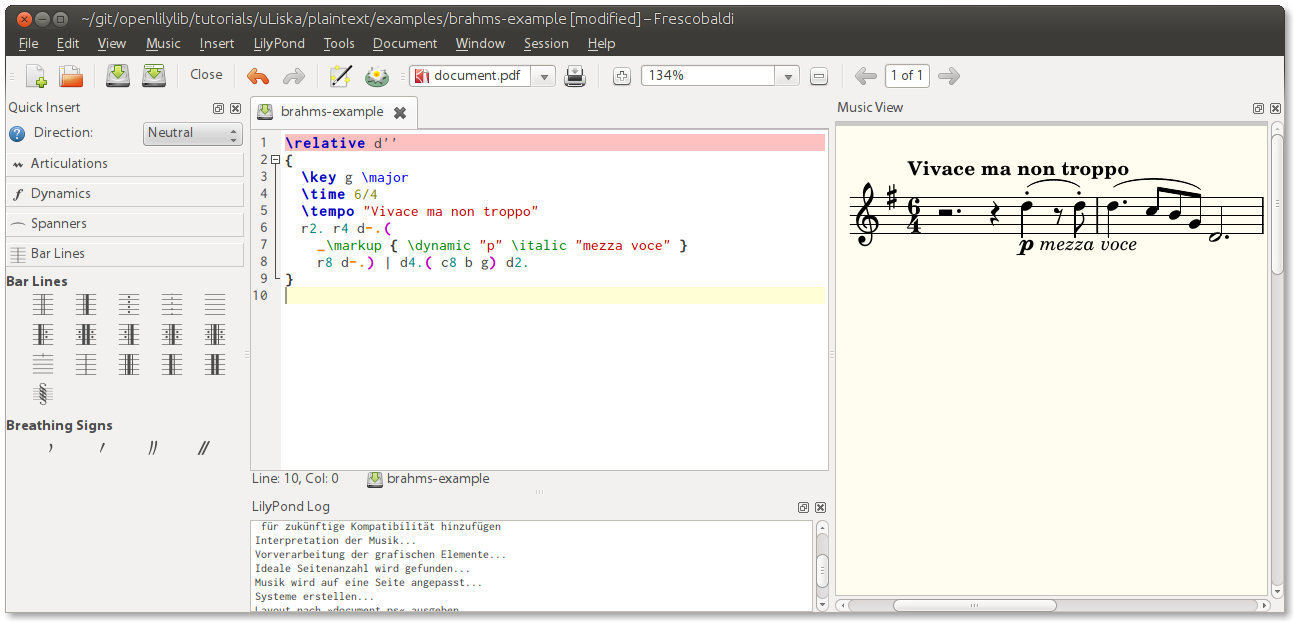
\includegraphics[max width=\textwidth]{examples/frescobaldi/main-window}
\caption{Frescobaldi's Main Window}
\label{fig:pt_fb-main-window}
\end{figure}

Another example of the useful tools is the \emph{Score Setup Wizard} that allows you to graphically configure a score of arbitrary complexity (just like in other programs) and that generates the text used for the corresponding score for you (see \fref{fig:pt_fb-score-setup-wizard}).

\begin{figure}
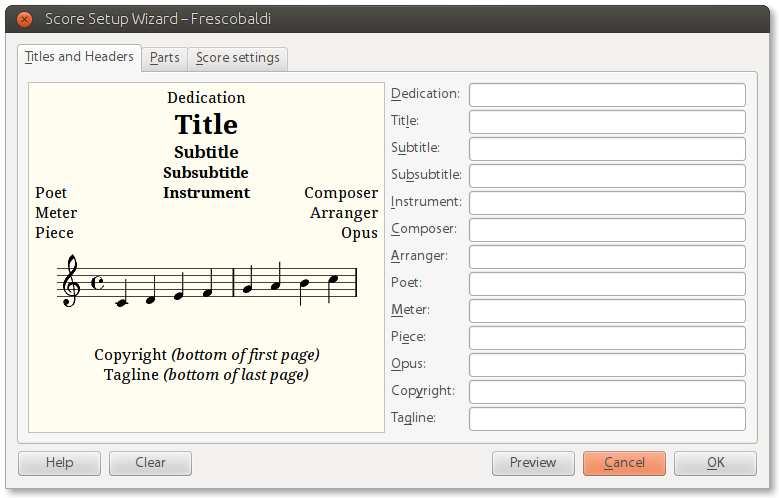
\includegraphics[max width=\textwidth]{examples/frescobaldi/score-wizard}
\caption{Frescobaldi: Score Setup Wizard}
\label{fig:pt_fb-score-setup-wizard}
\end{figure}

If you look at the text editor again (in \fref{fig:pt_fb-main-window}) you will see that the text is colored a lot (I will talk about the actual text soon).
This is a feature that Frescobaldi shares with most programming editors: it “knows” LilyPond's language and highlights the source text according to its structure.
Once one has got used to that practice it greatly eases reading and writing the necessary text files.

When you start typing a command Frescobaldi can also make suggestions on how to complete them (\fref{fig:pt_fb-code-completion})---also a valuable assistance, not so much because of its time-saving but because it assists you in remembering and efficiently reduces errors.

\begin{figure}
\centering
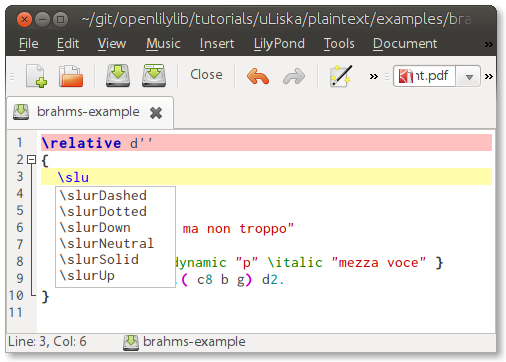
\includegraphics[width=8cm]{examples/frescobaldi/code-completion}
\caption{Frescobaldi: Suggestions for available commands}
\label{fig:pt_fb-code-completion}
\end{figure}

But maybe the most important feature for daily work is that you can click on an element in the music view and will be taken to the corresponding place in the input file.
In \fref{fig:pt_fb-point-and-click} you can see the slur highlighted in purple in the music view and the highlighted text in line 8 in the text editor.
\begin{figure}
\centering
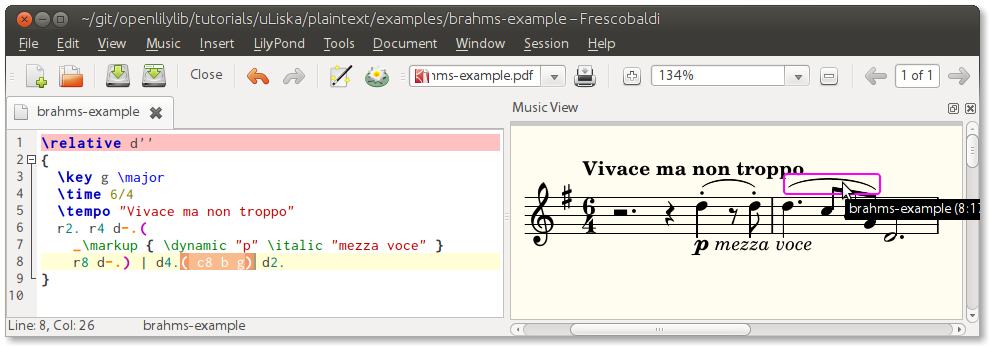
\includegraphics[max width=\textwidth]{examples/frescobaldi/point-and-click}
\caption{Frescobaldi: Two-way link between input file and score}
\label{fig:pt_fb-point-and-click}
\end{figure}
This also works in the other direction: If you select text in the editor the corresponding notation elements are highlighted in the score.
This lets you easily navigate your text file(s) and removes a handicap one could have seen in editing plain text files in the past.

One focus of current Frescobaldi development is the enhancement of the music view's functionality.
So it will soon be possible to partially “edit” the score with the mouse---of course in fact you will be able to tweak something visually and Frescobaldi will insert the appropriate text in the source file, possibly giving you the option to select from different approaches.
Currently there are plans to implement (e.\,g.) correcting pitches, drawing and shaping curves, and annotating objects (see also \fref{sec:pt_lilypond-comments}).
This will make “working with text files” even more comfortable.

Of course these remarks were only a very cursory overview of Frescobaldi.
A thorough introduction can't be the intention of this paper, but I wanted to give you a feeling to what extent current and smart editors can smoothen your editing experience.
Now you are ready to learn something about how LilyPond input files actually work.

\section{Textual Representation of Music}
\label{sec:pt_textual-representation}
In \fref{fig:pt_fb-main-window} (and \fref{fig:pt_fb-point-and-click}) you have seen a short score excerpt from Brahms' first violin sonata, along with the LilyPond code that produced it.
Now I'll use that example to show you a little bit about the basic elements in a LilyPond score.

At the most basic level notes are represented by their pitch and duration, as you can see in this “bare” example:

\begin{multicols}{2}
\begin{Verbatim}[samepage=true,
				   commandchars=|„“]
{
  r2. r4 d r8 d
  d4. c8 b g d2.
}
\end{Verbatim}
\columnbreak
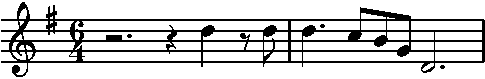
\includegraphics{examples/brahms/brahms-1}
\end{multicols}

The text writes rests (\texttt{\textit{r}}) and pitches (\texttt{\textit{d}} etc.) as well as durations (8, 4, 4., 2.), and everything is enclosed in a pair of curly braces.
This is LilyPond's notion of a \emph{music expression}.
A score is represented by one big music expression which can be constructed of arbitrarily nested or chained smaller music expressions.
There are a few things “missing” in the source that LilyPond adds by itself, namely a staff, a clef, and beams.

Two more elements aren't actually figured out automatically, but hidden from the example.
In fact you have to write down \cmd{key g} \cmd{major} and \cmd{time 6/4} to tell LilyPond about the key and time signatures.
But the beaming in the second measure is done automatically according to the time signature.
Many things can be defined by such \emph{commands}.

Elements like articulations or dynamics are attached to notes or rests by printing them after the reference item, like in this fake example:

\newcommand{\hilite}[1]{\textcolor{red}{\textbf{#1}}}

\begin{multicols}{2}
\begin{Verbatim}[samepage=true,
				   commandchars=|„“]
{
  r2. r4 d|hilite„-.“ r8 d|hilite„-.“ 
  d4.|hilite„\sf“ c8|hilite„\>“ b g|hilite„\!“ d2.|hilite„->“
}
\end{Verbatim}
\columnbreak
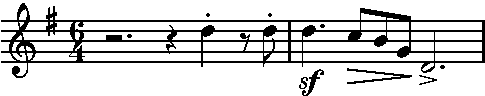
\includegraphics{examples/brahms/brahms-2}
\end{multicols}

We have a few articulations that are attached with a hyphen, the staccato dot written as a dot, the accent as a \texttt{>}, all characters have been chosen to be as intuitive as possible.
Dynamics are attached by a backslash, in the example we have the \lilyDynamics{sf} with \cmd{sf}, the \decrescHairpin with \cmd{>}, and (as the only unusual item) the \cmd{!} which represents the \emph{end} of the hairpin.

We can attach \emph{spanners} to pairs of notes, e.\,g.\ the slurs in the following example.
Slurs are written as opening and closing round brackets (\emph{after} the note they are referring to)
There you can see that you can attach multiple items to a note by just writing them one after another

\begin{multicols}{2}
\begin{Verbatim}[samepage=true,
				   commandchars=|„“]
{
  r2. r4 d-.|hilite„(“ r8 d-.|hilite„)“
  d4.|hilite„(“ c8|hilite„[“ b|hilite„]“ g|hilite„)“ d2.
}
\end{Verbatim}
\columnbreak
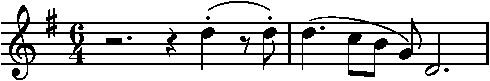
\includegraphics{examples/brahms/brahms-3}
\end{multicols}

In addition to the slurs you can also see an example of manually setting the beams against the rules for the time signature, which is indicated by the use of square brackets (again \emph{after} the notes they are referring to).

In the last example of this \emph{very} short introduction to LilyPond files we'll add the necessary text elements to the score.
The \emph{tempo} indication is entered by the \cmd{tempo} command (the non-verbal part is here as an example only), while the \lilyDynamics{p} \emph{mezza voce} is a \cmd{markup}---a text that is attached to a note like any articulation or dynamic sign.

\begin{multicols}{2}
\begin{Verbatim}[samepage=true,
				   commandchars=|„“]
{
  |hilite„\tempo“ "Vivace ma non troppo" |hilite„2. = 60“
  r2. r4 d-.(|hilite„-\markup“
    { \dynamic "p" \italic "mezza voce" } 
    r8 d-.) 
  d4.( c8 b g) d2.
}
\end{Verbatim}
\columnbreak
\vspace*{4.5em}
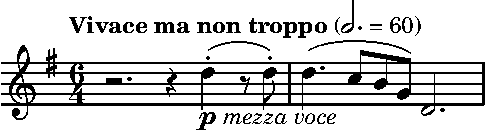
\includegraphics{examples/brahms/brahms-4}
\end{multicols}

One thing you may have noticed in the example is that I have broken the first line of music into three.
LilyPond doesn't care about this \emph{white space} and allows you to lay out your text file as you find appropriate---which usually will mean to keep coherent entities on a single line.
In this case the entity is the \emph{markup}, also an expression enclosed in curly braces.
You could just throw some text in there, but in this score we format the elements, one using the dynamics font, the other as italic text.

\medskip
Now you've seen your first real-world example of a LilyPond score.
Of course the complexity of these text files increases when the music gets longer or more complex.
But when looking at an input file you should always keep in mind that it is built from very small and rather simple units.
And you should feel comfortable with knowing that there are editors at hand that really help you navigating and editing them.

\section{Variables and Includes}
\label{sec:pt_variables-includes}
In the previous section I wrote that LilyPond adds necessary elements to what you have entered.
In the case of a file just consisting of a music expression as in our example it will actually add the necessary context for a staff, the score, and a “book” which represents the output file.
This works only for simple scores such as music examples or maybe plain chants, but for most real scores you will have to define the score structure explicitely.
While one would perhaps start with writing the music expressions directly inside the score set-up, there is the concept of \emph{variables} that proves infinitely useful for any project of some dimensions.

The basic structure of a score looks like this:
\begin{quote}
\begin{verbatim}
\score {
  \new Staff { ... music expression ... }
  \layout{}
  \midi{}
}
\end{verbatim}
\end{quote}

Inside the score block there is one \emph{Staff} that contains a music expression (I could have pasted the code from the previous examples here). \cmd{layout\{\}} tells LilyPond to create a score, the optional \cmd{midi\{\}} block additionally creates a \textsc{midi} file.
Instead of just \cmd{new Staff} there would be the complete structure of all (potentially nested) staves of the score, so the file would soon become very complex and confusing.
To avoid this one wraps up the music definition in a variable (e.\,g.\ \texttt{violin = \{ ... music ... \}}) and simply writes \verb+\new Staff \violin+ in the score block.

\medskip
Reading this you might consider it just a detail of the input file structure and wonder how this relates to you.
But packaging musical expressions in variables isn't only useful to reduce the complexity of the score block but serves many more goals.
It is a way for transparently and robustly store, use \emph{and reuse} blocks of music.
Reusing music is very useful, not only for the---admittedly quite specific---case of musical snippets or patterns, but also for the fundamental handling of the needs of musical engraving.
Earlier I wrote about the separation of content and appearance, here we are dealing with separation of the \emph{definition} and \emph{use} of music.
Music defined in a variable is used by a score---and it can equally be used by another score.
Different scores accessing shared music may be a full score and the instrumental parts or different transpositions of the same song.
In both cases the music is defined only once, and any update to that definition is propagated to all scores automatically.

Being able to reuse variables would only be a partial advantage if one couldn't separate the definitions even one step further, into separate files, and \emph{include} them.
This way one can create a collection of files, a \emph{library}, and keep them available for further use.
This is not only useful for reusing work in future projects but also within one project.
You can organize style and layout templates (i.\,e.\ definitions that influence the page layout and the appearance of the music) in a hierarchical and sophisticated way and have all files share some common styles (like font selections) but have different additional styles for different output formats (full score, part, music example \dots).
Any change in one of the style files is then automatically propagated to all scores.
Or you can make use of a technique called \emph{commenting out}---place two alternative includes but make a comment of one of them, like this:

\begin{Verbatim}
\include "draft-layout.ily"
%\include "publish-layout.ily"
\end{Verbatim}

The second line of this is a \emph{comment}, so only the draft-layout file will be included (and may color editorial additions red, print additional information about the date or whatever you like to define) as long as you are working on the score.
When you're finished and prepare the final printout you can just move the percent sign one line up and get your final publication layout.
And if you have this construction in a shared style file this switch will have global affect to all scores that are part of your project.

\section{Comments}
\label{sec:pt_lilypond-comments}
The last example of the previous section led us smoothly to the next aspect: \emph{comments}.
LilyPond---as virtually all plain text formats---allows you to mark parts of a file as comments, text that will be ignored by the typesetting.
This can for example be used to document what you have done or comment on technical issues you are facing.
You could for example explain why you have decided to implement a certain voice-leading to solve a typographic problem, or leave a mark that some issues will have to be resolved.
Combine this with the fact that all your manual interventions are written explicitely in the file and compare that with the situation of a graphical score editing program where you can hardly even tell what your manual interventions were \dots

Currently there are plans to greatly enhance this functionality, especially with preparing scholarly editions in mind.
It will be possible to enter specific comments in the input file---\emph{i.\,e.\ directly beside the music they are referring to}---and a tool that will be called \texttt{lilypond-doc} will output them to a variety of formats.
This will provide you with nicely formatted lists of 
\begin{inparaenum}
\item \textsc{todo} items,
\item musicological questions,
\item typographical questions, and finally
\item critical remarks.
\end{inparaenum}
The items in the list will be smartly linked, so that clicking on them will point you directly to the corresponding place in the source file.
\emph{Frescobaldi} will probably be able to allow you to insert such comments directly from within the music view, so you can click on a note and enter the comment.
This way you will be able to do all your work \emph{within the actual score} (and collectively with your collaborators), and finally you will get the entries for the critical report nicely sorted and formatted as source text to be used in the corresponding \LaTeX{} document!

\section{Conclusion}
\label{sec:pt_lilypond-conclusion}
By now it surely won't make you wonder that I wholeheartedly endorse the use of LilyPond as a notation software.
I can't recommend highly enough to give it at least a try---but you should give it a fair try and expect some time and effort needed initially.
From my experience (as a beginner and from seeing other beginners) I may give you some advice on \emph{do}s and \emph{don't}s:

Do \emph{not} jump right in and try to accomplish a complex project that has to be finished in time, or you will surely run into frustrations.
Ideally you should first read and follow the „Learning Manual“%
\footnote{\url{http://www.lilypond.org/doc/v2.16/Documentation/learning/index.html}}
from LilyPond's excellent documentation which will introduce you smoothly to the basic concepts.
But you may also tackle a task that is „real“ and on your desktop already.
This will make it more interesting, but be sure that it isn't too complex and that you won't run into having deliver it urgently.

Be sure \emph{not} to try it completely on your own, alone with you, the documentation and forum entries.
The ideal way would be to have someone mentoring you, giving you the right ideas and giving the right answers to the questions that really matter at a time.
Of course this isn't available for most of the beginners, so be sure to sign up to the lilypond-user mailing list%
\footnote{\url{https://lists.gnu.org/mailman/listinfo/lilypond-user}}.
Reading the discussion there (and skipping what seems too complicated for now) will be helpful to get a feeling for it, and the community is usually very responsive and helpful, as long as you show interest and own efforts.

Be sure to get used to using the documentation.
As mentioned it is excellent, but apart from the Learning Manual it is a \emph{reference} that mostly won't guide you through the concepts.
You will have to read things more than once, and for the starting time you will need to lookup things quite often.
Even later you will need to have good access to that reference.
So you should make yourself acquainted with the layout of the documentation as soon as possible.

\medskip
Admittedly it takes some time and effort to get productive with LilyPond.
But the benefits clearly outweigh that in my opinion.

First of all you instantly get beautiful output that is pleasing the eye.
LilyPond's very existence is due to the frustration two musicians had with the anemic sheet music they were confronted day to day on their orchestral music stands.
Therefore LilyPond's first ideal and models are traditional, hand-engraved scores, and you (and your readers) will benefit from that saturated page impression out of the box and in each score.
Practically this means that you will have \emph{significantly less work} to tune a score to be usable as performance material than when creating it with the known graphical programs (or the other way round: If you don't do that work at all (as obviously many composers do) the resulting material will be vastly superiour).
If you want to prepare scores for publication you will probably have to spend time with LilyPond too, applying a smaller number of corrections which will take more time each than with the graphical programs.
But as explained these corrections are much more robust, can be tracked and modified with a clean interface.

The other aspect of output quality is at least as important:
Since you get \emph{usable} results by default you can concentrate on the content much longer and only care about engraving details when actually preparing the final printout for publication.
But \emph{if} you want to apply manual modifications while still working on the content you have them in a clean and traceable way, and they won't step in the way when the final beautification takes place.

But what really sets working with LilyPond apart is the potential of new workflows powered by the plain text approach, as I have described in the previous chapters.
Seamlessly integrating work with others through versioning, documenting your work \emph{in situ}, setting up sophisticated and cascading style sheets on „house“, project or file level are the keywords to be mentioned here.
Interfacing scores or examples with \LaTeX{} documents will be one more topic, to be discussed in the next chapter.

\medskip
It wouldn't be honest to conceal one issue that I haven't touched so far: LilyPond's behaviour towards exchanging documents with other software.
Currently using LilyPond is kind of a one-way street with the only exit being the score in one of the various graphical output formats.
There are several ways to export/convert documents from other programs to be engraved by LilyPond (although you should expect some manual work to be done), but you can't simply export LilyPond input files to formats that can be used by other programs.
This usually isn't an issue when you are just creating scores to be printed, such as performance or teaching material, or music examples for books.
But it can be a show-stopper if you are preparing editions for commercial publishing houses because the majority of them has their established workflows and insists on getting the scores delivered as Finale\texttrademark{} or Sibelius\texttrademark{} files.
As you surely can imagine by now I wouldn't ever want to miss the plain text approach in preparing editions, so I would prefer doing it that way even if I knew (and felt sorry about it) that the score would end up being printed by one of the two programs.
So at least for this application it is a big desideratum to get LilyPond to export to MusicXML, a common interchange format.
As it stands, it doesn't even seem to be a major rewrite of the program but rather a few months of programmer's work.
Maybe \emph{one} rather large project with a sufficiently large organisation capable of bringing up some money would be enough to fix the situation.
But unfortunately there can't be any promises when (and if at all) this hole will be closed.

\chapter{\LaTeX}
\label{chap:pt_latex}

\LaTeX{} is for typesetting text documents what LilyPond is for typesetting scores.
It provides typesetting as opposed to mere text processing, providing the usual document author---who doesn't know too much about the rules of typography---with the necessary expertise to produce professionally typeset documents.
And it works by compiling plain text input files, so everything I have written about the advantages of using plain text files applies to \LaTeX{} equally.
Therefore I won't get into details introducing you to the concrete syntax of its input files, but try to introduce you concisely to some of the specifically musical features.

\LaTeX{} is available in form of \emph{distributions} such as \emph{TeXLive} for Linux, \emph{MacTeX} for Mac OS, or \emph{MiKTeX} for Windows.
These distributions are based on a number of core programs that actually perform the compilation of the input files.
In addition they contain numerous \emph{packages} that can be used to extend the typesetting capabilities.
Your interface to \LaTeX{} is the same as to LilyPond:
The input files can be edited with \emph{any} editor, and the compilers are command line programs.
But there are (quite numerous) dedictaed editors or IDEs%
\footnote{Integrated Development Environments}
that assist you in editing the documents and organizing the compilation process for you.

Earlier in \fref{sec:pt_separation-content-meaning-appearance} I showed you a basic \LaTeX{} document in which you saw the three fundamental elements: the \emph{document class}, \emph{commands} and \emph{environments} (although I didn't explicitely name the latter).
As mentioned the document class is somewhat comparable to a document template in an office application.
But it is much more powerful in that it can contain many layout elments, commands and more functionality.
The LaTeX{} distribution contains many document classes for many purposes (from standard articles over beamer presentations to classes specific to fields of research), but you can also download classes from other sources, and you can (and will) write your own.
One important aspect of document classes is the selection of \emph{packages} to be included.

When run on a basic document as in our example \LaTeX{} only loads a small subset of its possibilities in order to save time and memory.
If you need additional functionality you can include it through the use of \emph{packages}.
Such a package might contain anything from a small set of related semantic markup commands up to sophisticated bibliographic functionality%
\footnote{See \url{http://en.wikibooks.org/wiki/LaTeX/Package_Reference} for a list of some packages with short comments on their functionality}.
When you want a different style for tables or lists, to include images, or add music examples---chances are good that there is a package enabling just what you need.

As I have also mentioned earlier the \emph{commands} and \emph{environments} are roughly similar to character and paragraph styles as used in office documents.
But they too are much more powerful because they are more like programmer's commands, especially as they use arguments.
A command can do anything with its arguments which makes it a very versatile tool.
As a single example I have a command for entries in a revision report that takes arguments for measure number, position in the measure, affected voice/system, and the actual comment.
This information it then processed to a nice layout, skipping the separator characters when an argument is empty.
If I should decide upon a completely different layout I just have to update the command to propagate it to the whole document---or a complete set of documents if I have defined it in a package.
And of course I will soon be able to incorporate the report entries that \texttt{lilypond-doc} will give me from within the LilyPond scores \dots

\emph{Environments} are somewhat similar, with the difference that the commands are a one-time event while environments have a begin and an end (like the \emph{document environment} seen in the initial example).
Environments like \env{figure} or \env{table} allow you to place graphical items as \emph{floating} objects.
This allows \LaTeX{} to place them at the best position concerning the page breaking.
While this is something one has to get used to it is actually a big enhancement towards a \emph{professional} typesetting, especially of books and similar documents.
As producing books is the basic motivation for \LaTeX{} you also can expect professional tools with regard to bibliography, indices or figure lists etc.

\medskip
Now that we have seen a \emph{very} short introduction to \LaTeX{} it is time to consider some specifically \emph{musical} aspects to authoring text documents.

\section{Music Examples}
\label{sec:pt_music-examples}
Of course you can embed images in text documents if you want to add music examples to a text.
\LaTeX{} does a very good job at typesetting these additions with the best possible quality.
But there are a few dedicated tools that aid you with this specific task, in particular I will talk about \package{lilypond-book} and \package{musicexamples}.

\subsection{lilypond-book}
\label{subsec:pt_lilypond-book}
The program \package{lilypond-book} is part of the LilyPond distribution and allows to embed LilyPond source code directly in \LaTeX{} documents.
First you run \package{lilypond-book} on the document, which will call LilyPond to generate all (necessary) examples and create a copy of the document including these generated files.
Then you run \LaTeX{} to compile this processed copy.
This procedure has some overhead due to the large number of intermediate files, and many people using \package{lilypond-book} with complex documents or on a regular basis actually approach this using self-made scripts.
But if you have documents with lots of (small) examples you won't find any better solution to manage your music sources \emph{in situ}.

\subsection{musicexamples}
\label{subsec:pt_musicexamples}
Another way to embed music examples in \LaTeX{} documents is \package{musicexamples}, a package that is part of \openlilylib%
\footnote{\url{http://www.openlilylib.org/musicexamples}}.
Originally started as an alternative approach to \package{lilypond-book} it can actually work together with it quite well.
\package{musicexamples} provides environments and commands to include and manage music examples in \LaTeX{} documents.
There is support for floating and non-floating environments, single-line or multi-line examples (with the multi-line ones being able to be split on several pages).
You can also print full-page examples, with special support for examples starting on odd or even pages (you can force an example to start at the next odd or even page).
All examples in a document share the same counter and can be exported to a contigious list of music examples.

It is possible to use \emph{any} images for your music examples, but there is special support for using LilyPond (of course).
There are tools compiling your LilyPond files to files that can directly be used in the \LaTeX{} document, especially taking care of the odd/even issue.
This may be the way for you if you want to manage your scores separately from the text document.
Finally there will be%
\footnote{This part of the package hasn't been implemented yet.}
helper scripts that keep the music examples up to date (and conditionally recompile missing music example files).

Instead of existing image files (LilyPond generated or not) you can equally embed LilyPond code with \package{lilypond-book} and benefit from both approaches:
\package{lilypond-book}s in-place example code and \package{musicexamples}' beautiful layout and example management.

You can see a comprehensive example document with music examples in the appendix \todo{fref}.

\subsection{OOoLilyPond}
\label{subsubsec:pt_ooo-lilypond}
Finally I have to mention another option to integrate music examples in text documents, although it isn't quite as professional.
\emph{OOoLilyPond%
\footnote{\todo{URL}}}
is an OpenOffice extension which allows to store LilyPond code as embedded objects in Writer documents.
It can compile them in place and display the corresponding image files while keeping the source code ready for further editing.
Unfortunately this can only produce bitmaps and no vector graphics, resulting in a rather medium output quality.

\section{Notational Elements}
\label{sec:pt_notational-elements}
Another member of our family of resources is \lilyglyphs[scale=1.1].
This package allows to include LilyPond's notational elements in the continuous text of \LaTeX{} documents.
This is significantly different from entering music examples as it will embed them as characters, like \lilyDynamics{mf} for example.
The main advantage of this package over any other solution I know of is that these elements are readily available, scale well with the surrounding text size, and that you can realize virtually anything you can do with LilyPond.

Elements that are part of LilyPond's OpenType font can be accessed through predefined commands (the above example was written \cmd{lilyDynamics\{mf\}}) or---if there isn't a predefined command yet---through their glyph names from the font, like this \lilyGlyph[scale=1, raise=0.75]{clefs.mensural.c} mensural clef \cmd{lilyGlyph{\{clefs.mensural.c\}}}.

For elements that aren't part of the OpenType font and that are normally drawn by LilyPond \lilyglyphs[scale=1.1] uses small images that have been generated with LilyPond.
The use is identical if there are predefined commands like this \crotchet[scale=1.1] \cmd{crotchet} or other non-text \crescHairpin  elements.
If there isn't a predefined command or if you need a very non-standard symbol, \lilyglyphs[scale=1.1] assists you in creating your own predefined commands with a relatively easy to use interface:
You will provide a small “template file”, and a tool will manage the process for you up to generating the necessary \LaTeX{} command.
This way you can include arbitrary notational elements as characters in your text documents, with perfect control over the scaling and positioning.

\section{Conclusion}
\label{sec:pt_latex-conclusion}

If you care at all about typography and write text documents you should love \LaTeX. 
If you don't care about typography you should know that typography \emph{is} effective even if you didn't intend it.
Typography can't be absent, usually it's just \emph{bad} typography then.
Therefore documents should be created with good tools.
\LaTeX{} produces good typography, word processors don't, period.
DTP programs like InDesign\texttrademark{} or QuarkXPress\texttrademark{} can be used to create good-looking documents, but they are very expensive, and especially for long documents they are significantly less efficient.
If you add to that the described possibilities to integrate text and music and especially the potentials of versioning and collaboration you should see that \LaTeX{} is definitely worth giving a try.
If you are already acquainted with LilyPond the learning curve won't be as steep anymore, although it surely needs some change of mind when coming from office applications.

If you have to deliver documents in other forms than \textsc{pdf} files (usually office files that hopefully are typeset with professional tools afterwards) you still can benefit from the versioning part which improves your efficiency---
I wouldn't want to work any other way by now.
Other than LilyPond scores \LaTeX source files can be exported to a variety of formats like \textsc{rtf} or \textsc{html}.
This process isn't always guaranteed, though---the more sophisticated your tools and commands are the more problems will arise with export filters.
Which should be evident: If you design complex custom commands with multiple arguments, how should a converter know to translate them to \textsc{rtf} for example?
So if you write program notes that have to be delivered as a Word file you can still use \LaTeX{} to author the document but keep it simple in terms of layout or structure.
But this isn't really a restriction because if you're working in such a context you are usually expected to deliver “raw” material anyway.

\chapter{Applications}
\label{chap:pt_applications}

\section{Preparing a Musical Edition}
\label{sec:pt_preparing-edition}
This is what I actually experienced recently---and what I definitely don't want to miss anymore.
There are several steps in preparing a scholarly edition, which are partly interdependent and are partly distributed between different team members.
\begin{itemize*}
    \item Entering the music
    \item Setting up the score layout and the style sheets
    \item Proof-reading the music
    \item Scholarly revision
    \item Fine-tuning the engraving
    \item Authoring critical reports
    \item Layout of the main volume and prepress
\end{itemize*}
With the described plain text tools all of these steps can be done within one code base.
While it would traditionally also be done in one file there is a major difference: the code base is shared and continuously accessible by everybody, the single (binary) score file can only be shared consecutively, with complicated and risky workflows to avoid unrecoverable conflicts.
The technical infrastructure doesn't impose any restrictions on the workflow and order of the steps beyond what is immanent in the task (it doesn't make sense for example to fine-tune the engraving while there are still revisions in process that might change the content).
When an editor finds an error just before the edition is sent to the printer he may simply correct it \emph{in the shared code base}, and the engraver can immediately check for side-effects and fix these if necessary.

\section{Book preparation}
The same is true for the preparation of books, and of compilation books from more than one author in particular.
All collaborators can seamlessly work together in a shared code base: the author(s), editors, typesetters, and maybe additional specialists preparing figures or music examples.
A collaborative set-up provides for an efficient workflow between an author and his editor, and it can be particularly useful when proof-reading or documents or polishing them linguistically with many assistants.

\section{Single-source Publishing}
\label{sec:pt_single-source-publishing}

Plain text files are a good starting point for creating documents for different output formats.
One example already discussed is the possibility to create several different scores (or parts) with LilyPond from a single set of input files.
But this can quite easily be extended to generating documents for printing, beamer presentation, mobile devices and web pages from single sources.

\todo{more/better examples?}

\section{“Crowd Editing”}
\label{sec:pt_crowd-editing}

A last use case is something that isn't really common yet because it can exclusively be inspired by the use of workflows that are driven by version control.
With the capability to manage contributions by a (practically) unlimited number of participants it is possible to create musical scores with a large community.
This way the workload can be “clustered” among a potentially great number of people, each one according to his capabilities and special knowledge (about specific instruments for example), and large quantities of music entered in astonishingly little time.
While this doesn't save actual working hours it can be used to process them in parallel.
Even in a large-scale symphonic score each single part is quite manageable, and if there is one contributor for each part (or better: two contributors for two parts who do a peer-review before submitting) the score should grow rapidly.
In such a context the aspect of programmability may once more become important.
The “project” may be supported by extensive programming without the individual contributor knowing anything about it---it may even be explicitely programmed to expose the individual to a quite simple interface.


\chapter{Where To Go From Here?}
\label{chap:pt_where-to-go-from-here}

\todo{Recommended introductory material for the individual aspects}

\appendix
\chapter{Appendix}

\begin{itemize}
\item \todo{Binary/plain text file comparisons}
\item \todo{\lilyglyphs example document}
\item \texttt{musicexamples} example document
\end{itemize}
\includepdf[%
	pages=-]{../../../musicexamples/documentation/example-document/xmp-Example}
\end{document}